\documentclass[../../ThesisDoc]{subfiles}
% \documentclass{standalone}
%
% \usepackage{tikz, ifthen}
% \usetikzlibrary{fit, matrix, positioning, shapes, decorations.pathreplacing,
%                 shapes.geometric, chains, arrows, calc }

\begin{document}


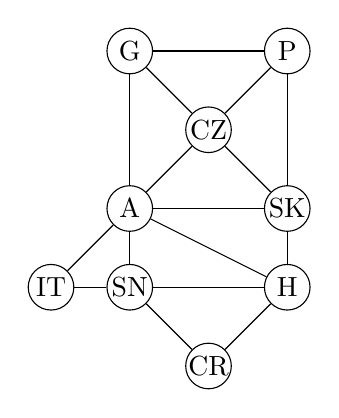
\begin{tikzpicture}[
  every node/.style={draw, circle, inner sep=0pt, text width=1.5em, align=center}
  ]

\node (IT) at (0,0)   {IT};
\node (SN) at (1,0)   {SN};
\node (CR) at (2,-1)  {CR};
\node (H)  at (3,0)   {H};
\node (A)  at (1,1)   {A};
\node (SK) at (3,1)   {SK};
\node (CZ) at (2,2)   {CZ};
\node (G)  at (1,3)   {G};
\node (P)  at (3,3)   {P};

\draw (G) -- (P);
\draw (G) -- (CZ);
\draw (G) -- (A);
\draw (P) -- (CZ);
\draw (P) -- (SK);
\draw (CZ) -- (A);
\draw (CZ) -- (SK);
\draw (A) -- (SK);
\draw (A) -- (H);
\draw (A) -- (SN);
\draw (A) -- (IT);
\draw (SK) -- (H);
\draw (IT) -- (SN);
\draw (SN) -- (H);
\draw (SN) -- (CR);
\draw (H) -- (CR);

\end{tikzpicture}
\end{document}
